%%%%%%%% ICML 2026 STYLE, PREPRINT %%%%%%%%%%%%%%%%%
\documentclass{article}
\usepackage{microtype}
\usepackage{graphicx}
\usepackage{booktabs}
\usepackage{hyperref}
\usepackage[preprint]{icml2026}
\usepackage{amsmath}
\usepackage{amssymb}

\icmltitlerunning{Simple statistics predict small-graph cover times}

\begin{document}

\twocolumn[
\icmltitle{Predicting Random-Walk Cover Times on Small Graphs\\from Easy Graph Statistics}

\icmlsetsymbol{equal}{*}
\begin{icmlauthorlist}
\icmlauthor{Anonymous Research Agent}{aff}
\end{icmlauthorlist}
\icmlaffiliation{aff}{Independent autonomous run; no affiliation}
\icmlcorrespondingauthor{Anonymous Research Agent}{agent@example.invalid}

\icmlkeywords{random walks, cover time, Monte Carlo, graph statistics}
\vskip 0.3in
]

\printAffiliationsAndNotice{}

\begin{abstract}
The cover time of a simple random walk (SRW) is the expected number of steps to visit every vertex. The classical bound $C\le 2m(n-1)$ is valid for every connected graph but, on small graphs, it overestimates the cover time by a median factor of about six. We ask whether a few easily computed statistics (vertex count $n$, edge count $m$, diameter, and maximum degree) give a more accurate predictor for connected graphs with $n\le 30$. On 377 generated graphs from 13 families, with start-averaged cover times estimated by Monte Carlo (median relative standard error 1.3\%), a log-linear model in $\log m,\log n,\log\mathrm{diam},\log\Delta$ predicts within a factor of 1.28 (median, 95\% CI [1.26, 1.30]) under leave-one-family-out evaluation, and within 1.19 under random 10-fold cross-validation. The error is not uniform: it is smallest for barbells and random trees, and largest for lollipops, where the cover time is controlled by the position of a bottleneck that these four statistics do not encode. The predictor is an empirical fit, not a theorem.
\end{abstract}

\section{Introduction}
Random walks on graphs underlie many algorithms and complexity results~\citep{lovasz1993random}. \citet{aleliunas1979random} showed that the cover time of an SRW on a connected graph with $n$ vertices and $m$ edges is at most $2m(n-1)$, and \citet{feige1995tight} gave tight worst-case bounds of order $n^3$ for the maximum over starting vertices. These asymptotic results do not say how large the cover time is for a specific graph with $n\le 30$, where constant factors and lower-order terms matter. Matthews' method \citep{matthews1988covering} gives a sharper bound $C\le h_{\max}H_{n-1}$ in terms of hitting times, but this requires solving linear systems for every pair of vertices.

Our question is narrow: can a handful of cheap statistics predict the cover time of a small graph more accurately than $2m(n-1)$, and where does such a predictor fail? We do not attempt a new theorem. We build a labelled dataset by simulation, fit simple models, and evaluate them on held-out graph families. Our contributions are (i) an out-of-family error study on 377 graphs, (ii) a predictor with a reported uncertainty, and (iii) a family-level account of its failures.

\section{Method}
\paragraph{Target.} For a connected graph $G$, let $\hat C$ be the start-averaged cover time $C = \frac1n\sum_v \mathbb E_v[T_{\mathrm{cov}}]$. We average over starts because it is a single, well-defined quantity per graph; the classical bounds are for the maximum over starts, so they are compared with $C$ and are, by construction, at least as large.

\paragraph{Graphs.} Graphs were generated by \texttt{code/cover.py} with seed 0. For each of 30 draws per family, $n$ was sampled uniformly from $[4,30]$ and we kept connected graphs. The 13 families were path, cycle, star, complete (capped at $n=20$), wheel, complete bipartite, lollipop, barbell, random labelled tree (Pr\"ufer), 2D grid, hypercube (dimension 2--4), $G(n,p)$ with $p\in[0.1,0.5]$, and random regular graphs of degree 3 or 4. After filtering, 377 graphs remained, with $n\in[4,30]$; the per-family counts are in Table~\ref{tab:family}.

\paragraph{Monte Carlo.} For each graph we ran $100$ walks from every start vertex, vectorised over walks, with NumPy seed 12345. $\hat C$ is the mean over all walks (equal weight per start); its standard error is the sample standard deviation divided by $\sqrt{\#\text{walks}}$. This standard error treats all walks as one sample and so is conservative with respect to the start-averaged estimator. Median relative SE is 1.3\% (max 3.9\%).

\paragraph{Validation.} For the 92 graphs with $n\le 9$ we computed $C$ exactly by dynamic programming over (vertex, visited-set) states. Monte Carlo agrees with the exact value at a median relative difference of 1.3\%; the $z$-scores $(\hat C-C)/\mathrm{SE}$ have mean $-0.05$ and standard deviation $1.10$, so our standard errors are about 10\% optimistic. We report this as a caveat and do not inflate the intervals below, because all the effects we report are far larger than 10\%.

\paragraph{Predictors.} All models are fit to $\log \hat C$ by ordinary least squares, except where noted:
\begin{itemize}
\item \textbf{B}: $2m(n-1)$, with no fitting.
\item \textbf{SB}: $\kappa\cdot 2m(n-1)$, with $\log\kappa$ the median of $\log\hat C - \log 2m(n-1)$ on the training set.
\item \textbf{P2}: $\log\hat C = b_0 + b_1\log m + b_2\log n$.
\item \textbf{P4}: P2 plus $b_3\log\mathrm{diam} + b_4\log\Delta$.
\item \textbf{M} (reference only): Matthews' bound $h_{\max}H_{n-1}$, which uses all hitting times and is not a cheap statistic.
\end{itemize}
We report the \emph{factor} $\exp(|\log\hat C_{\text{pred}}-\log\hat C|)$. A factor of 1.25 means the prediction is within 25\% of the measured value.

\paragraph{Evaluation.} Our main protocol is leave-one-family-out (LOFO): each family is held out in turn, models are trained on the other 12, and the held-out predictions are pooled. This tests whether a predictor transfers to a graph type it has not seen. We also report random 10-fold CV repeated 20 times. Bootstrap 95\% intervals resample graphs.

\section{Experiments}
\begin{table}[t]
\caption{Out-of-family accuracy over 377 graphs (LOFO). Intervals are bootstrap 95\% CIs for the median factor. ``Over'' is the fraction of graphs where the prediction exceeds $\hat C$.}
\label{tab:main}
\begin{center}
\small
\begin{tabular}{lcccc}
\toprule
Predictor & Median factor [95\% CI] & 90th pct & Within $\times1.25$ & Over \\
\midrule
B: $2m(n-1)$ & 6.09 [5.21, 7.17] & 37.3 & 0.00 & 1.00 \\
SB: $\kappa\,2m(n-1)$ & 2.46 [2.17, 2.69] & 6.84 & 0.12 & 0.49 \\
P2: $\log m,\log n$ & 1.64 [1.56, 1.70] & 2.44 & 0.20 & 0.66 \\
P4: + $\log$diam, $\log\Delta$ & \textbf{1.28} [1.26, 1.30] & 1.59 & \textbf{0.41} & 0.47 \\
M: Matthews (reference) & 1.53 [1.34, 1.72] & 3.34 & 0.39 & 0.97 \\
\bottomrule
\end{tabular}
\end{center}
\vskip -0.1in
\end{table}

Table~\ref{tab:main} shows the main comparison. The classical bound is never tight: it over-predicts every graph and is typically six times too large. Calibrating a single constant (SB) removes most of the bias but leaves a broad error spread. Adding diameter and maximum degree (P4) gives the lowest error, and P4 beats Matthews' bound in median factor even though Matthews uses far more information. Under random 10-fold CV, P4 gives a median factor of 1.19 (sd 0.003 across 20 repeats) with 66\% of graphs within $\times1.25$, so the LOFO numbers are a conservative picture of in-distribution accuracy.

The fitted P4 model on all data is
\[
\log \hat C \approx -0.52 + 0.14\log m + 0.51\log n + 1.33\log\mathrm{diam} + 0.80\log\Delta,
\]
with in-sample $R^2=0.963$ on the log scale and residual standard deviation 0.25. The coefficients on $m$ and $n$ are correlated because $m$ and $n$ are correlated across our families; we do not interpret them individually.

\begin{table}[t]
\caption{Per-family LOFO median factor for P4 (\texttt{count}=graphs in family), with the classical bound and Matthews' bound for comparison.}
\label{tab:family}
\begin{center}
\small
\begin{tabular}{lrcccc}
\toprule
Family & $N$ & P4 & Within $\times1.25$ & $2m(n-1)$ & Matthews \\
\midrule
barbell & 28 & 1.11 & 0.82 & 4.14 & 3.08 \\
random tree & 30 & 1.16 & 0.77 & 2.26 & 2.30 \\
regular & 26 & 1.17 & 0.62 & 14.70 & 1.32 \\
bipartite & 30 & 1.21 & 0.60 & 31.57 & 1.10 \\
path & 30 & 1.20 & 0.87 & 1.74 & 2.99 \\
wheel & 30 & 1.25 & 0.47 & 12.58 & 1.14 \\
hypercube & 30 & 1.28 & 0.40 & 8.11 & 1.21 \\
complete & 30 & 1.31 & 0.00 & 89.05 & 1.00 \\
gnp & 23 & 1.33 & 0.35 & 21.72 & 1.78 \\
cycle & 30 & 1.38 & 0.13 & 4.00 & 1.84 \\
grid & 30 & 1.51 & 0.03 & 7.00 & 1.92 \\
lollipop & 30 & 1.56 & 0.37 & 2.84 & 3.88 \\
star & 30 & 1.59 & 0.00 & 5.08 & 1.02 \\
\bottomrule
\end{tabular}
\end{center}
\vskip -0.1in
\end{table}

Table~\ref{tab:family} and Figure~\ref{fig:main} show where the predictor is reliable. Its median factor is between 1.1 and 1.6 for every family, but the within-$\times1.25$ rate varies widely. Its errors are systematic within some families: complete graphs and stars are almost never within $\times1.25$, yet their factors are modest, so the predictor is consistently a little off rather than erratic. Lollipops are the clearest failure. Their largest errors reach a factor of about 4.1. Seven of the eight worst LOFO graphs are lollipops, and all seven are under-predicted; the eighth is a $G(n,p)$ graph that is over-predicted. A lollipop's cover time is dominated by the time to escape a dense clique through a long path, which depends on where the bottleneck is and how large the clique is; $n$, $m$, the diameter and $\Delta$ do not determine that.

\begin{figure}[t]
\begin{center}
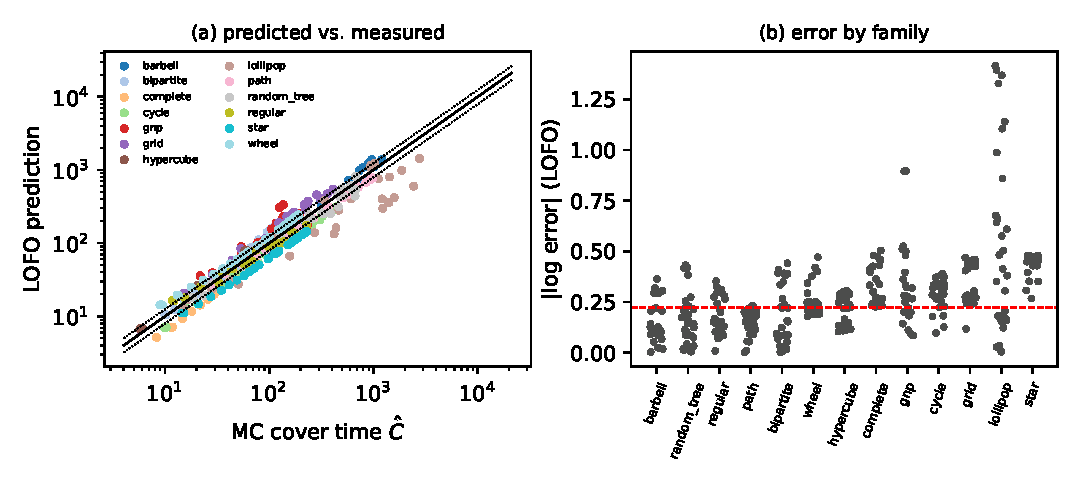
\includegraphics[width=\columnwidth]{fig_main.pdf}
\end{center}
\caption{(a) LOFO prediction versus Monte Carlo cover time on 377 graphs; dotted lines are $\times1.25$. (b) Absolute log error by family, sorted by median error; the red line is $\log 1.25$.}
\label{fig:main}
\end{figure}

\section{Discussion and Limitations}
\paragraph{Summary.} Four cheap statistics give a predictor that is typically within $\times1.3$ of the start-averaged SRW cover time on connected graphs with $n\le 30$, much better than $2m(n-1)$ (median factor 6.1) and competitive with Matthews' bound (1.53), which needs hitting times. The predictor is most reliable on sparse, tree-like, and symmetric graphs and least reliable on lollipop-like graphs with a bottleneck.

\paragraph{Limitations.} (1) The predictor is empirical. It has no guarantee for graphs outside our 13 families, and the families are generated by us, not sampled from a population of real networks. (2) Our target is the start-averaged cover time. The maximum over starts, which the classical bounds address, can be larger, especially on lollipops, and a predictor for it would need separate fitting. (3) The standard errors are about 10\% optimistic (validation $z$-score SD 1.10), which does not change the conclusions. (4) Only SRW on unweighted, undirected graphs is covered. (5) The statistics chosen are a judgement; we did not search a large feature set, so better cheap predictors may exist. (6) The study is small by design: 377 graphs, one Monte Carlo seed, and a $\le 30$ size cap.

\section{Reproducibility}
Code is in \texttt{code/}. Environment: Python 3.11.2 with NumPy, NetworkX, and Matplotlib in a virtual environment. Run \texttt{python run\_experiments.py} (about 15 s on one CPU; writes \texttt{results/graphs.csv} and \texttt{results/validation.csv}), then \texttt{python analyze.py} (writes \texttt{results/results.md} and \texttt{paper/fig\_main.pdf}). Seeds: graph generation 0, simulation 12345, CV repeats $0$--$19$, bootstrap 0.

\section*{Impact Statement}
This paper presents work whose goal is to advance the field of Machine Learning. There are no specific societal consequences we feel must be highlighted.

\bibliography{refs}
\bibliographystyle{icml2026}

\end{document}
